\documentclass[a4paper]{article}

\usepackage[top=1in, bottom=1.25in, left=1.25in, right=1.25in]{geometry}
\usepackage{graphicx}
\usepackage{amsmath}
\usepackage{amssymb}
\usepackage[sorting=none]{biblatex}
\usepackage{warning} % for warning messages

\usepackage{url}
\usepackage{microtype}
\usepackage{lmodern}
\usepackage[colorlinks=true, citecolor=red, linkcolor=blue]{hyperref}

\usepackage{caption}
\usepackage{subcaption}
\usepackage{float}
\usepackage{booktabs}
\usepackage{multirow}
\usepackage[affil-it]{authblk}

\usepackage{todonotes}

\usepackage{siunitx}

\usepackage[compat=1.1.0]{tikz-feynman} % generate feynman diagrams

\bibliography{references}
\overfullrule=2cm % allows to find overfull hboxes much quicker

\binoppenalty=3000
\relpenalty=3000

\title{Applications of Standard Model Effective Field Theory to 2D differential distributions of top pair production}
\author{Alexander Veltman\\{\small Advisor: Dr.\ James Keaveney}}
\affil{Department of Physics,\\University of Cape Town}

\begin{document}
\maketitle

\begin{abstract}
\end{abstract}

\section{Introduction}

\begin{itemize}
    \item Standard model is good
    \item Cannot explain some phenomena
    \item New frame work called SMEFT
\end{itemize}

\section{LHC, ATLAS and Top Physics}

\begin{figure}[h]
    \centering
    \feynmandiagram[horizontal=a to b] {
        i1 -- [gluon] a -- [gluon] i2,
        a -- [gluon] b,
        f1 [particle=$\bar{t}$] -- [fermion] b -- [fermion] f2 [particle=$t$],
    };
    \caption{Top Quark Pair production}
\end{figure}


\section{Standard Model Effective field theory}

Standard Model effective field theory (SMEFT) is a model-independent framework for identifying and constraining deviations from Standard Model predictions.
This is done by considering that some higher mass particles or higher energy reactions may exist and seeing the imprints on regular Standard Model cross-sections and interactions.
The framework introduces a set of dimension-six terms into the Standard Model Lagrangian which only contains operators of dimension-four.
These includes 59 independent operators (according to what is known as the Warsaw basis) which are built from Standard Model fields and follow the gauge symmetries of the Standard Model \cite{Grzadkowski_2010}.


With the additional operators, the SMEFT Lagrangian is
\begin{equation}\label{eq:smeft_lagrangian}
    \mathcal{L}_{\text{SMEFT}} = \mathcal{L}_{\text{SM}} + \frac{1}{\Lambda^2} \sum\limits_{i} C_{i} O_{i} + \mathcal{O}\left(\frac{1}{\Lambda^3}\right)
\end{equation}
where $O_{i}$ is a dimension-six operator and $C_{i}$ is an associated dimensionless coupling constant known as a \emph{Wilson Coefficient}.
The operators are reduced by the energy scale $\Lambda$ of the BSM physics.

These effects manifest themselves in observable cross sectional data \cite{Hartland_2019}

\begin{equation}\label{eq:smeft_cross_section}
    \sigma = \sigma_{\text{SM}} + \sum\limits_{i} \frac{1}{\Lambda^2} C_{i} \sigma_{i} + \sum\limits_{j,k} \frac{1}{\Lambda^4} C_{j} C_{k} \sigma_{j k}
\end{equation}
where $\sigma$ is an integrated cross section.

The effects on differential cross section with respect to an observable are similar
\begin{equation}\label{eq:smeft_diff_cross_section}
    \frac{d\sigma}{dX} = \frac{d\sigma}{dX}_{\text{SM}} + \sum\limits_{i} \frac{1}{\Lambda^2} C_{i} \frac{d\sigma_{i}}{dX} + \sum\limits_{j,k} \frac{1}{\Lambda^4} C_{j} C_{k} \frac{d\sigma_{j k}}{dX}
\end{equation}

Using (\ref{eq:smeft_diff_cross_section}), the influences of SMEFT can be identified within differential cross section measurements obtained through modern collider experiments.

\todo{link to top physics}
\todo{Talk about relevant operators to top production}

\begin{figure}
    \centering
    \begin{subfigure}[b]{0.20\textwidth}
        \feynmandiagram [small, horizontal=a to b] {
            i1 [particle=$\bar{q}$] -- [fermion] a -- [gluon] b [dot] -- [fermion] f1 [particle=$t$],
            i2 [particle=$q$] -- [anti fermion] a,
            b   -- [anti fermion] f2 [particle=$\bar{t}$],
        };
    \end{subfigure}
    \hfill
    \begin{subfigure}[b]{0.20\textwidth}
    \feynmandiagram [small, vertical=a to b] {
        i1 [particle=$g$] -- [gluon] a [dot] -- [fermion] f1 [particle=$t$],
        i2 [particle=$g$] -- [gluon] b [dot] -- [anti fermion] f2 [particle=$\bar{t}$],
        b -- [fermion] a,
    };
    \end{subfigure}
    \hfill
    \begin{subfigure}[b]{0.20\textwidth}
    \feynmandiagram [small, vertical=i1 to i2] {
        i1 [particle=$g$] -- [gluon] a [dot] -- [fermion] f1 [particle=$t$],
        i2 [particle=$g$] -- [gluon] a -- [anti fermion] f2 [particle=$\bar{t}$],
        i1 -- [opacity=0] i2,
        f1 -- [opacity=0] f2,
    };
    \end{subfigure}
    \hfill
    \begin{subfigure}[b]{0.20\textwidth}
    \begin{tikzpicture}
        \begin{feynman}
            \vertex (a);
            \vertex [above left=1cm of a] (i1) {$q$};
            \vertex [above right=1cm of a] (f1) {$t$};
            \vertex [below left=1cm of a] (i2) {$\bar{q}$};
            \vertex [below right=1cm of a] (f2) {$\bar{t}$};
        \diagram* {
            (i1) -- [fermion] (a) [dot] -- [fermion] (f1),
            (i2) -- [anti fermion] (a) -- [anti fermion] (f2),
        };
        \end{feynman}
    \end{tikzpicture}
    \end{subfigure}

    \caption{Examples of leading order diagrams which contribute to top pair production in SMEFT}
\end{figure}

\section{dEFT}
\todo{dEFT bio}

\subsection{Model building}
dEFT creates predictions for the observables of interest for varying values of Wilson coefficients by constructing a morphing model.
A morphing model is a linear regression model which allows for the interpolation between different templates.
These templates are Monte Carlo predictions which are generated around the region of parameter space which would be relevant for some dataset.
For dEFT's application, cross sectional SMEFT predictions which are generated using some event generation framework are used as templates.
These predictions must describe the relevant set of operators $O_{i}$ with varying Wilson Coefficients in order to produce a reliable model.
Using $\ref{eq:smeft_cross_section}$, a linear model is constructed using these templates and produces a predictive model $\hat{\sigma}({C_i})$.
This model now allows for the prediction of some cross sectional observable for any values of Wilson coefficients pertaining to the relevant set of operators.

\subsection{Fitting Method}
\todo{talk about MCMC}
\todo{Benefits of MCMC over likelihood minimisation}
\todo{talk about Smefit methods}

\section{Analysis}

\todo{Talk about ATLAS dataset}

\subsection{Monte Carlo event generation}
In order to build the morphing model required to generate cross sectional predictions, simulated samples are required throughout the space of Wilson coefficients of the operators of interest.
These samples were generate using the MadGraph5\textunderscore aMC@NLO~\cite{Alwall_2014} framework which allows for the simulation of processes for a user-defined Lagrangian.
The SMEFTatNLO~\cite{degrande2020automated} FEYNRULES model implements SMEFT tree level and one loop processes into MadGraph5.
Though there is the capacity to perform predictions at next-to-leading order, these calculations are very recent \todo{Justify why LO better} and greatly increase the processing time required to produce the Monte Carlo predictions.
The simulations are performed to fixed order where only the desired observables of $m_{t\bar{t}}$ and ${p_{T}^{t}}$ are calculated and binned in the same binning arrangement as the ATLAS dataset \todo{need to mention ATLAS dataset before this point}.

\subsubsection{\texorpdfstring{$k$}{k}-factor determination}
Since the generated Monte Carlo samples only included LO processes, theses predictions needed to be scaled to be comparable to the necessary data sets.
It can be considered fairly accurate to compare NNLO predictions to actual cross sectional data so a method of scaling the current predictions to this level is required.
Due to the difficulty in calculating the $k$-factor for different combinations of Wilson coefficients values, the $k$-factor for the Standard Model prediction was used across the various SMEFT predictions.

A flat $k$-factor across the differential cross sections was attempted to bring the LO predictions to the scale of NNLO predictions using the proportions between tree level calculations of total cross section~\cite{Alwall_2014} and measurement of total cross section using the ATLAS detector~\cite{ATLAS:2019hxz}.
This method failed due to some regions of the differential cross sections being poorly described at LO which caused a flat scaling to incorrectly describe the shape of the distributions at NNLO.
This is exemplified by the low $m_{t\bar{t}}$ and high $p_{T}^{t}$ region in our two observable data set, as seen in Figure~\ref{fig:kfactor}.
This is remedied by requiring a per-bin $k$-factor when scaling from LO to NLO but still using the flat factor to build up to NNLO.
The per-bin $k$-factor was found by comparing the Standard Model predictions of MadGraph5 at LO and NLO and applying this ratio to the Monte Carlo signal.
The theoretical error associated with the calculated $k$-factor is fairly difficult to propagate through the model construction and should be dominated by the error associated with the data.
This may have consequences on bins which are not well described at LO though the scale variances in these regions should dominate the theoretical uncertainties.

\begin{figure}
    \centering
    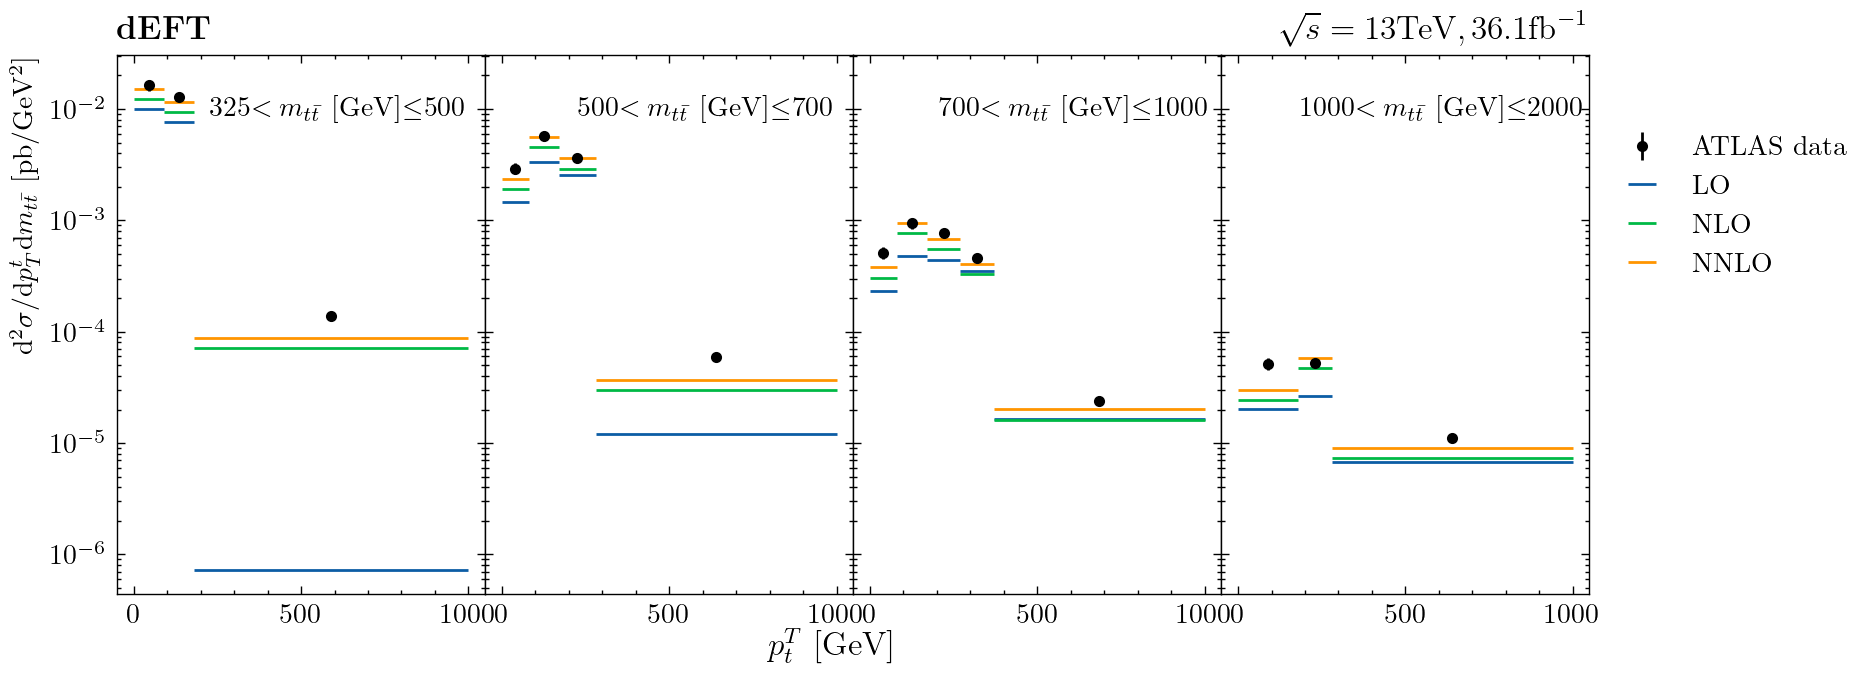
\includegraphics[width=0.8\textwidth]{plots/k_factor.png}
    \caption{Comparison of approximations of levels of prediction for processes contributing to absolute double differential $t\bar{t}$ cross section with respect to $m_{t\bar{t}}$ and $p_{T}^{t}$. The scaling from LO to NLO was determined using a per-bin method and the NNLO prediction was determined using a flat factor.}
    \label{fig:kfactor}
\end{figure}


\subsection{\texorpdfstring{$m_{t\bar{t}}$}{mttbar} differential cross section}
\subsubsection{Model Validation}
\subsubsection{Results}

\subsection{Double differential cross section}
\subsubsection{Model Validation}
\subsubsection{Results}

\section{Conclusion}

\newpage
\begingroup
\raggedright{}
\sloppy
\printbibliography{}
\endgroup

\end{document}
